\section{Исследование четырёхразрядного синхронного суммирующего
счётчика с параллельным переносом на Т-триггерах.}

Ниже, на рисунке \ref{sc1}, представлена схема четырехразрядного счетчика на Т-триггерах.

\begin{figure}[ht]
    \centering
    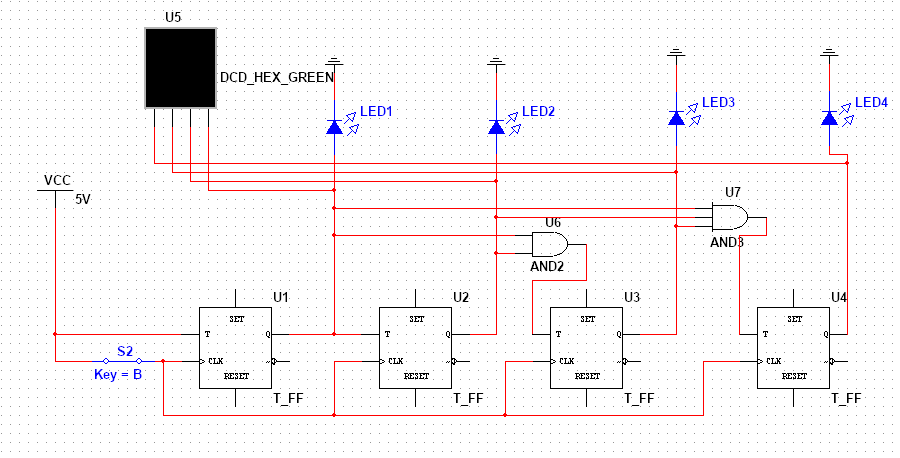
\includegraphics[width=\linewidth]{img/sc1.png}
    \caption{Схема четырёхразрядного счётчика на T-триггерах}
    \label{sc1}
\end{figure}

При каждой итерации замыкания-размыкания, счетчик увеличивается на один, лампочки указывают двоичное представление полученного числа, а дисплей шестнадцатеричное.

\begin{figure}[ht]
    \centering
    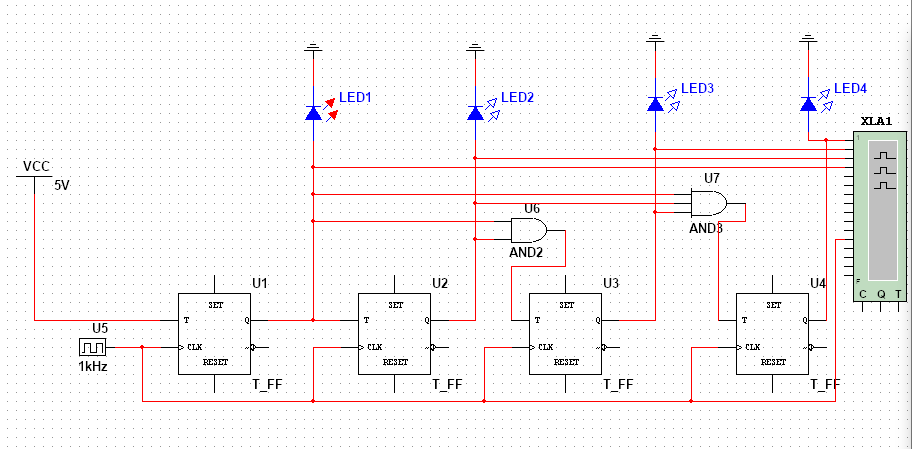
\includegraphics[width=\linewidth]{img/sc2.png}
    \caption{Схема четырёхразрядного счетчика с логическим анализатором}
    \label{sc2}
\end{figure}

Ниже представлена временная диаграмма, полученная с помощью импульсного генератора и логического анализатора сигналов.

\begin{figure}[ht]
    \centering
    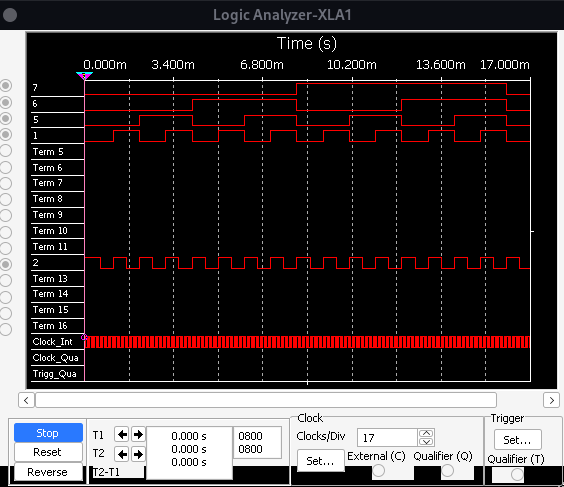
\includegraphics[width=0.7\linewidth]{img/sc3.png}
    \caption{Временная диаграмма четырёхразрядного счётчика на T-триггерах}
    \label{sc3}
\end{figure}

\clearpage

\section{Синтез двоично-десятичного счётчика с заданной последовательностью состояний}

Последовательность состояний: (0, 1, 2, 4, 5, 6, 10, 11, 13, 14)

Ниже представлена таблица возбуждений сигналов JK и ее процесс минимизации.

\begin{center}
	\begin{tabular}{ | l | l | l | l | l | l | l | l | l | l | l | l | l | l | l | l | p{1cm} |}
		\hline
	 	$Q_{3}$ & $Q_{2}$ & $Q_{1}$ & $Q_{0}$ & $Q_{3}*$ & $Q_{2}*$ & $Q_{1}*$ & $Q_{0}*$ & $J_{3}$ & $K_{3}$ & $J_{2}$ & $K_{2}$ & $J_{1}$ & $K_{1}$ & $J_{0}$ & $K_{0}$ \\\hline
	 	0 & 0 & 0 & 0 & 0 & 0 & 0 & 1 & 0 & $\lambda$ & 0 & $\lambda$ & 0 & $\lambda$ & 1 & $\lambda$ \\\hline
	 	0 & 0 & 0 & 1 & 0 & 0 & 1 & 0 & 0 & $\lambda$ & 0 & $\lambda$ & 1 & $\lambda$ & $\lambda$ & 1 \\\hline
	 	0 & 0 & 1 & 0 & 0 & 1 & 0 & 0 & 0 & $\lambda$ & 1 & $\lambda$ & $\lambda$ & 1 & 0 & $\lambda$ \\\hline
	 	- & - & - & - & - & - & - & - & - & - & - & - & - & - & - & - \\\hline
	 	0 & 1 & 0 & 0 & 0 & 1 & 0 & 1 & 0 & $\lambda$ & $\lambda$ & 0 & 0 & $\lambda$ & 1 & $\lambda$ \\\hline
	 	0 & 1 & 0 & 1 & 0 & 1 & 1 & 0 & 0 & $\lambda$ & $\lambda$ & 0 & 1 & $\lambda$ & $\lambda$ & 1 \\\hline
	 	0 & 1 & 1 & 0 & 1 & 0 & 1 & 0 & 1 & $\lambda$ & $\lambda$ & 1 & $\lambda$ & 0 & 0 & $\lambda$ \\\hline
	 	- & - & - & - & - & - & - & - & - & - & - & - & - & - & - & - \\\hline
	 	- & - & - & - & - & - & - & - & - & - & - & - & - & - & - & - \\\hline
	 	- & - & - & - & - & - & - & - & - & - & - & - & - & - & - & - \\\hline
	 	1 & 0 & 1 & 0 & 1 & 0 & 1 & 1 & $\lambda$ & 0 & 0 & $\lambda$ & $\lambda$ & 0 & 1 & $\lambda$ \\\hline
	 	1 & 0 & 1 & 1 & 1 & 1 & 0 & 1 & $\lambda$ & 0 & 1 & $\lambda$ & $\lambda$ & 1 & $\lambda$ & 0 \\\hline
	 	- & - & - & - & - & - & - & - & - & - & - & - & - & - & - & - \\\hline
	 	1 & 1 & 0 & 1 & 1 & 1 & 1 & 0 & $\lambda$ & 0 & $\lambda$ & 0 & 1 & $\lambda$ & $\lambda$ & 1 \\\hline
	 	1 & 1 & 1 & 0 & 0 & 0 & 0 & 0 & $\lambda$ & 1 & $\lambda$ & 1 & $\lambda$ & 1 & 0 & $\lambda$ \\\hline
	 	- & - & - & - & - & - & - & - & - & - & - & - & - & - & - & - \\
		\hline
	\end{tabular}

    \pagebreak

	""\newline
	$J_{3} = q_{2} \& q_{1}$
	
	""\newline
	\begin{tabular}{ | l | l | l | l | l | p{1cm} |}
		\hline
		\diagbox[width=5em]{$q_{3}q_{2}$}{$q_{1}q_{0}$} & 00 & 01 & 11 & 10 \\\hline
		00 & 0 & 0 & - & 0 \\\hline
		01 & 0 & 0 & \cellcolor{blue!25} - & \cellcolor{blue!25} 1 \\ \hline
		11 & - & $\lambda$ & \cellcolor{blue!25} - &  \cellcolor{blue!25} $\lambda$ \\ \hline
		10 & - & - & $\lambda$ & $\lambda$ \\ 
		\hline
	\end{tabular}

	""\newline\newline
	$K_{3} = q_{2} \& q_{1}$
	
	""\newline
	\begin{tabular}{ | l | l | l | l | l | p{1cm} |}
		\hline
		\diagbox[width=5em]{$q_{3}q_{2}$}{$q_{1}q_{0}$} & 00 & 01 & 11 & 10 \\\hline
		00 & $\lambda$ & $\lambda$ & - & $\lambda$ \\\hline
		01 & $\lambda$ & $\lambda$ & \cellcolor{blue!25} - & \cellcolor{blue!25} $\lambda$ \\ \hline
		11 & - & 0 & \cellcolor{blue!25} - &  \cellcolor{blue!25} 1  \\ \hline
		10 & - & - & 0 & 0 \\ 
		\hline
	\end{tabular}

	""\newline\newline
	$J_{2} = (\overline{q_{3}} \& q_{1})| (q_{3} \& q_{0})$
	
	""\newline
	\begin{tabular}{ | l | l | l | l | l | p{1cm} |}
		\hline
		\diagbox[width=5em]{$q_{3}q_{2}$}{$q_{1}q_{0}$} & 00 & 01 & 11 & 10 \\\hline
		00 & 0 & 0 & \cellcolor{blue!25} - & \cellcolor{blue!25} 1 \\\hline
		01 & $\lambda$ & $\lambda$ & \cellcolor{blue!25} - & \cellcolor{blue!25} $\lambda$ \\ \hline
		11 & - & \cellcolor{blue!25} $\lambda$ & \cellcolor{blue!25} - &  $\lambda$  \\ \hline
		10 & - & \cellcolor{blue!25} - & \cellcolor{blue!25} 1 & 0 \\ 
		\hline
	\end{tabular}

	""\newline\newline
	$K_{2} = q_{1}$
	
	""\newline
	\begin{tabular}{ | l | l | l | l | l | p{1cm} |}
		\hline
		\diagbox[width=5em]{$q_{3}q_{2}$}{$q_{1}q_{0}$} & 00 & 01 & 11 & 10 \\\hline
		00 & $\lambda$  & $\lambda$  & \cellcolor{blue!25} - & \cellcolor{blue!25} $\lambda$  \\\hline
		01 & 0 & 0 & \cellcolor{blue!25} - & \cellcolor{blue!25} 1 \\ \hline
		11 & - &  0 & \cellcolor{blue!25} - &  \cellcolor{blue!25} 1  \\ \hline
		10 & - & - & \cellcolor{blue!25} \cellcolor{blue!25} $\lambda$  & \cellcolor{blue!25} $\lambda$  \\ 
		\hline
	\end{tabular}

	""\newline\newline
	$J_{1} = q_{0}$
	
	""\newline
	\begin{tabular}{ | l | l | l | l | l | p{1cm} |}
		\hline
		\diagbox[width=5em]{$q_{3}q_{2}$}{$q_{1}q_{0}$} & 00 & 01 & 11 & 10 \\\hline
		00 & 0  & \cellcolor{blue!25} 1  & \cellcolor{blue!25} - & $\lambda$  \\\hline
		01 & 0  & \cellcolor{blue!25} 1  & \cellcolor{blue!25} - & $\lambda$  \\\hline
		11 & 0  & \cellcolor{blue!25} 1  & \cellcolor{blue!25} - & $\lambda$  \\\hline
		10 & -  & \cellcolor{blue!25} - & \cellcolor{blue!25} $\lambda$  & $\lambda$  \\ 
		\hline
	\end{tabular}

	\clearpage
	$K_{1} = (q_{1} \& q_{0}) | (\overline{q_{3)}} \& \overline{q_{2}}) | (q_{3} \& q_{2})$
	
	""\newline
	\begin{tabular}{ | l | l | l | l | l | p{1cm} |}
		\hline
		\diagbox[width=5em]{$q_{3}q_{2}$}{$q_{1}q_{0}$} & 00 & 01 & 11 & 10 \\\hline
		00 & \cellcolor{blue!25} $\lambda$  & \cellcolor{blue!25} $\lambda$  & \cellcolor{blue!25} - & \cellcolor{blue!25} 1  \\\hline
		01 & $\lambda$  &  $\lambda$  & \cellcolor{blue!25} - & 0  \\\hline
		11 & \cellcolor{blue!25} -  & \cellcolor{blue!25} $\lambda$  & \cellcolor{blue!25} - & \cellcolor{blue!25} 1  \\\hline
		10 & -  & - & \cellcolor{blue!25} 1  & 0  \\ 
		\hline
	\end{tabular}

	""\newline\newline
	$J_{0} = \overline{q_{1}} | (q_{3} \& \overline{q_{2)}}$
	
	""\newline
	\begin{tabular}{ | l | l | l | l | l | p{1cm} |}
		\hline
		\diagbox[width=5em]{$q_{3}q_{2}$}{$q_{1}q_{0}$} & 00 & 01 & 11 & 10 \\\hline
		00 & \cellcolor{blue!25} 1  & \cellcolor{blue!25} $\lambda$  & - & 0  \\\hline
		01 & \cellcolor{blue!25} 1  & \cellcolor{blue!25} $\lambda$  & - & 0  \\\hline
		11 & \cellcolor{blue!25} 1  & \cellcolor{blue!25} $\lambda$  & - & 0  \\\hline
		10 & \cellcolor{blue!25} -  & \cellcolor{blue!25} - & \cellcolor{blue!25} $\lambda$  & \cellcolor{blue!25} 1  \\ 
		\hline
	\end{tabular}

	""\newline\newline
	$K_{0} = \overline{q_{1}}$
	
	""\newline
	\begin{tabular}{ | l | l | l | l | l | p{1cm} |}
		\hline
		\diagbox[width=5em]{$q_{3}q_{2}$}{$q_{1}q_{0}$} & 00 & 01 & 11 & 10 \\\hline
		00 & \cellcolor{blue!25} $\lambda$  & \cellcolor{blue!25} 1  & - & $\lambda$  \\\hline
		01 & \cellcolor{blue!25} $\lambda$  & \cellcolor{blue!25} 1  & - & $\lambda$  \\\hline
		11 & \cellcolor{blue!25} -  & \cellcolor{blue!25} 1 & - & $\lambda$  \\\hline
		10 & \cellcolor{blue!25} -  & \cellcolor{blue!25} - & 0  & $\lambda$  \\ 
		\hline
	\end{tabular}

\end{center}

Получаем схему на логических элементах и JK-триггерах: (рисунок \ref{sc4})

\begin{figure}[ht]
    \centering
    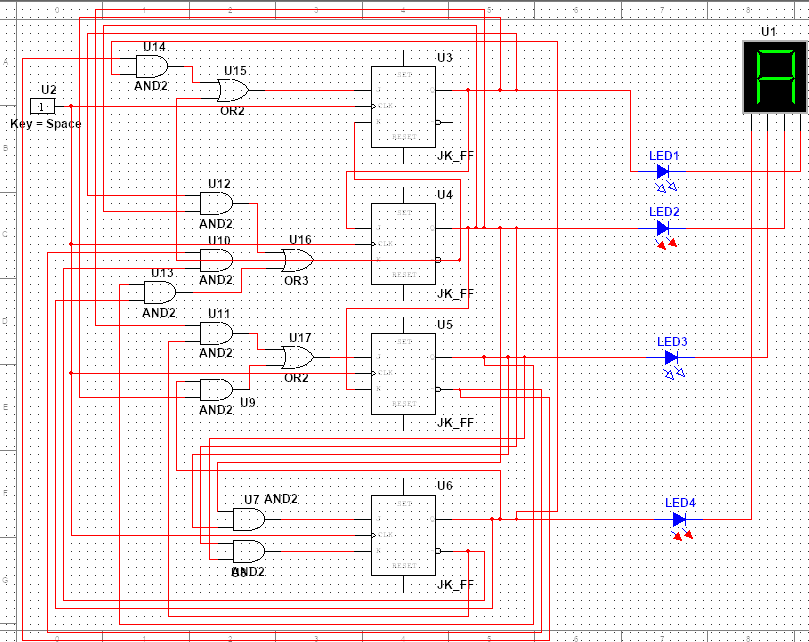
\includegraphics[width=\linewidth]{img/sc4.png}
    \caption{Временная диаграмма четырёхразрядного счётчика на T-триггерах}
    \label{sc4}
\end{figure}

\pagebreak

\section{Сбор десятичного счётчика на элементной базе приложения Multisim}

Минимизация и таблица:
\begin{center}
	\begin{tabular}{ | l | l | l | l | l | l | l | l | l | l | l | l | l | l | l | l | p{1cm} |}
		\hline
		$Q_{3}$ & $Q_{2}$ & $Q_{1}$ & $Q_{0}$ & $Q_{3}*$ & $Q_{2}*$ & $Q_{1}*$ & $Q_{0}*$ & $J_{3}$ & $K_{3}$ & $J_{2}$ & $K_{2}$ & $J_{1}$ & $K_{1}$ & $J_{0}$ & $K_{0}$ \\\hline
		0 & 0 & 0 & 0 & 0 & 0 & 0 & 1 & 0 & $\alpha$ & 0 & $\alpha$ & 0 & $\alpha$ & 1 & $\alpha$ \\\hline
		0 & 0 & 0 & 1 & 0 & 0 & 1 & 0 & 0 & $\alpha$ & 0 & $\alpha$ & 1 & $\alpha$ & $\alpha$ & 1 \\\hline
		0 & 0 & 1 & 0 & 0 & 0 & 1 & 1 & 0 & $\alpha$ & 0 & $\alpha$ & $\alpha$ & 0 & 1 & $\alpha$ \\\hline
		0 & 0 & 1 & 1 & 0 & 1 & 0 & 0 & 0 & $\alpha$ & 1 & $\alpha$ & $\alpha$ & 1 & $\alpha$ & 1 \\\hline
		0 & 1 & 0 & 0 & 0 & 1 & 0 & 1 & 0 & $\alpha$ & $\alpha$ & 0 & 0 & $\alpha$ & 1 & $\alpha$ \\\hline
		0 & 1 & 0 & 1 & 0 & 1 & 1 & 0 & 0 & $\alpha$ & $\alpha$ & 0 & 1 & $\alpha$ & $\alpha$ & 1 \\\hline
		0 & 1 & 1 & 0 & 0 & 1 & 1 & 1 & 0 & $\alpha$ & $\alpha$ & 0 & $\alpha$ & 0 & 1 & $\alpha$ \\\hline
		0 & 1 & 1 & 1 & 1 & 0 & 0 & 0 & 1 & $\alpha$ & $\alpha$ & 1 & $\alpha$ & 1 & $\alpha$ & 1 \\\hline
		1 & 0 & 0 & 0 & 1 & 0 & 0 & 1 & $\alpha$ & 0 & 0 & $\alpha$ & 0 & $\alpha$ & 1 & $\alpha$ \\\hline
		1 & 0 & 0 & 1 & 0 & 0 & 0 & 0 & $\alpha$ & 1 & 0 & $\alpha$ & 0 & $\alpha$ & $\alpha$ & 1 \\\hline
		- & - & - & - & - & - & - & - & - & - & - & - & - & - & - & - \\\hline
		- & - & - & - & - & - & - & - & - & - & - & - & - & - & - & - \\\hline
		- & - & - & - & - & - & - & - & - & - & - & - & - & - & - & - \\\hline
		- & - & - & - & - & - & - & - & - & - & - & - & - & - & - & - \\\hline
		- & - & - & - & - & - & - & - & - & - & - & - & - & - & - & - \\\hline
		- & - & - & - & - & - & - & - & - & - & - & - & - & - & - & - \\
		\hline
	\end{tabular}

    \pagebreak

	""\newline\newline
	$J_{3} = q_{0} \& q_{1} \& q_{2}$
	
	""\newline
	\begin{tabular}{ | l | l | l | l | l | p{1cm} |}
		\hline
		\diagbox[width=5em]{$q_{3}q_{2}$}{$q_{1}q_{0}$} & 00 & 01 & 11 & 10 \\\hline
		00 & 0 & 0  & 0 & 0  \\\hline
		01 & 0 & 0  & \cellcolor{blue!25} 1 & 0  \\\hline
		11 & - & -  & \cellcolor{blue!25} - & -  \\\hline
		10 & $\alpha$ & $\alpha$  & - & -  \\
		\hline
	\end{tabular}

	""\newline\newline
	$K_{3} = q_{0}$
	
	""\newline
	\begin{tabular}{ | l | l | l | l | l | p{1cm} |}
		\hline
		\diagbox[width=5em]{$q_{3}q_{2}$}{$q_{1}q_{0}$} & 00 & 01 & 11 & 10 \\\hline
		00 & $\alpha$ & \cellcolor{blue!25} $\alpha$  & \cellcolor{blue!25} $\alpha$ & $\alpha$  \\\hline
		01 & $\alpha$ & \cellcolor{blue!25} $\alpha$  & \cellcolor{blue!25} $\alpha$ & $\alpha$  \\\hline
		11 & - & \cellcolor{blue!25} -  & \cellcolor{blue!25} - & -  \\\hline
		10 & 0 & \cellcolor{blue!25} 1  & \cellcolor{blue!25} - & -  \\
		\hline
	\end{tabular}

	\clearpage
	$J_{2} = q_{0} \& q_{1}$
	
	""\newline
	\begin{tabular}{ | l | l | l | l | l | p{1cm} |}
		\hline
		\diagbox[width=5em]{$q_{3}q_{2}$}{$q_{1}q_{0}$} & 00 & 01 & 11 & 10 \\\hline
		00 & 0 & 0  & \cellcolor{blue!25} 1 & 0  \\\hline
		01 & $\alpha$ & $\alpha$ & \cellcolor{blue!25} $\alpha$ & $\alpha$  \\\hline
		11 & - & -  & \cellcolor{blue!25} - & -  \\\hline
		10 & 0 & 0  & \cellcolor{blue!25} - & -  \\
		\hline
	\end{tabular}

	""\newline\newline
	$K_{2} = q_{0} \& q_{1}$
	
	""\newline
	\begin{tabular}{ | l | l | l | l | l | p{1cm} |}
		\hline
		\diagbox[width=5em]{$q_{3}q_{2}$}{$q_{1}q_{0}$} & 00 & 01 & 11 & 10 \\\hline
		00 & $\alpha$ & $\alpha$  & \cellcolor{blue!25} $\alpha$ & $\alpha$  \\\hline
		01 & 0 & 0  & \cellcolor{blue!25} 1 & 0  \\\hline
		11 & - & -  & \cellcolor{blue!25} - & -  \\\hline
		10 & $\alpha$ & $\alpha$ & \cellcolor{blue!25} - & -  \\
		\hline
	\end{tabular}

	""\newline\newline
	$J_{1} = q_{0} \& \overline{q_{3}}$
	
	""\newline
	\begin{tabular}{ | l | l | l | l | l | p{1cm} |}
		\hline
		\diagbox[width=5em]{$q_{3}q_{2}$}{$q_{1}q_{0}$} & 00 & 01 & 11 & 10 \\\hline
		00 & 0 & \cellcolor{blue!25} 1  & \cellcolor{blue!25} $\alpha$ & $\alpha$  \\\hline
		01 & 0 & \cellcolor{blue!25} 1  & \cellcolor{blue!25} $\alpha$ & $\alpha$  \\\hline
		11 & - & -  & - & -  \\\hline
		10 & 0 & 0  & - & -  \\
		\hline
	\end{tabular}

	""\newline\newline
	$K_{1} = q_{0}$
	
	""\newline
	\begin{tabular}{ | l | l | l | l | l | p{1cm} |}
		\hline
		\diagbox[width=5em]{$q_{3}q_{2}$}{$q_{1}q_{0}$} & 00 & 01 & 11 & 10 \\\hline
		00 & $\alpha$ & \cellcolor{blue!25} $\alpha$  & \cellcolor{blue!25} 1 & 0  \\\hline
		01 & $\alpha$ & \cellcolor{blue!25} $\alpha$  & \cellcolor{blue!25} 1 & 0  \\\hline
		11 & - & \cellcolor{blue!25} -  & \cellcolor{blue!25} - & -  \\\hline
		10 & $\alpha$ & \cellcolor{blue!25} $\alpha$ & \cellcolor{blue!25} - & -  \\
		\hline
	\end{tabular}

	""\newline\newline
	$J_{0} = 1$
	
	""\newline
	\begin{tabular}{ | l | l | l | l | l | p{1cm} |}
		\hline
		\diagbox[width=5em]{$q_{3}q_{2}$}{$q_{1}q_{0}$} & 00 & 01 & 11 & 10 \\\hline
		00 & \cellcolor{blue!25} 1 & \cellcolor{blue!25} $\alpha$ & \cellcolor{blue!25} $\alpha$ & \cellcolor{blue!25} 1  \\\hline
		01 & \cellcolor{blue!25} 1 & \cellcolor{blue!25} $\alpha$ & \cellcolor{blue!25} $\alpha$ & \cellcolor{blue!25} 1  \\\hline
		11 & \cellcolor{blue!25} - & \cellcolor{blue!25} -  & \cellcolor{blue!25} - & \cellcolor{blue!25} -  \\\hline
		10 & \cellcolor{blue!25} 1 & \cellcolor{blue!25} $\alpha$  & \cellcolor{blue!25} - & \cellcolor{blue!25} -  \\
		\hline
	\end{tabular}

	\clearpage
	$K_{0} = 1$
	
	""\newline
	\begin{tabular}{ | l | l | l | l | l | p{1cm} |}
		\hline
		\diagbox[width=5em]{$q_{3}q_{2}$}{$q_{1}q_{0}$} & 00 & 01 & 11 & 10 \\\hline
		00 & \cellcolor{blue!25} $\alpha$ & \cellcolor{blue!25} 1 & \cellcolor{blue!25} 1 & \cellcolor{blue!25} $\alpha$  \\\hline
		01 & \cellcolor{blue!25} $\alpha$ & \cellcolor{blue!25} 1 & \cellcolor{blue!25} 1 & \cellcolor{blue!25} $\alpha$  \\\hline
		11 & \cellcolor{blue!25}- & \cellcolor{blue!25}-  & \cellcolor{blue!25} - & \cellcolor{blue!25} -  \\\hline
		10 & \cellcolor{blue!25} $\alpha$ & \cellcolor{blue!25}1  & \cellcolor{blue!25} - & \cellcolor{blue!25} -  \\
		\hline
	\end{tabular}
\end{center}

Получаем схему (рисунок \ref{sc5}) -- счетчик в двоично-десятичной системе счисления. По данной схеме можно строить счетчики произвольного порядка.

\begin{figure}[ht]
    \centering
    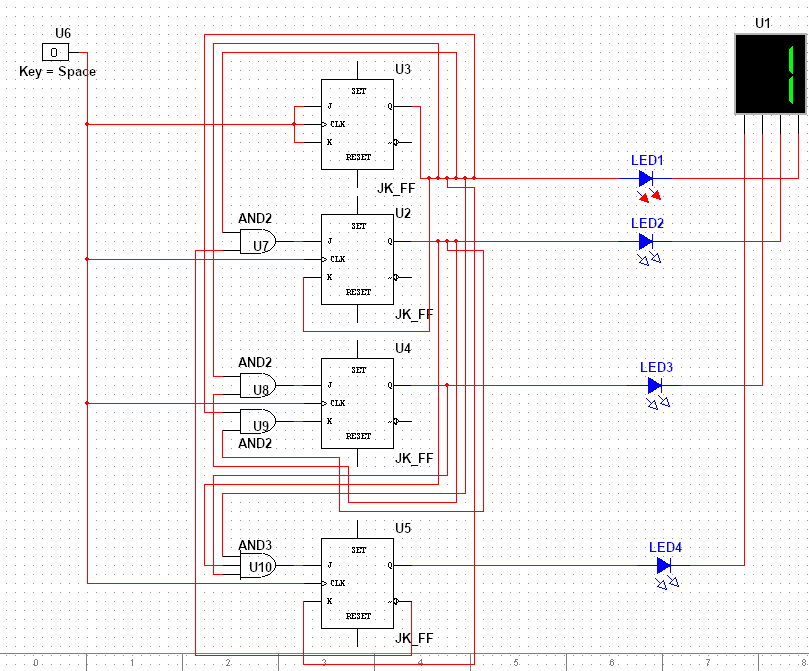
\includegraphics[width=\linewidth]{img/sc5.png}
    \caption{Схема десятичного счетчика на элементной базе Multisim.}
    \label{sc5}
\end{figure}

\section{Исследование четырёхразрядного синхронного суммирующего счётчика с параллельным переносом}

Ниже, на рисунке \ref{sc6}, представлена схема в шестнадцатеричной системе счисления.

\begin{figure}[ht]
    \centering
    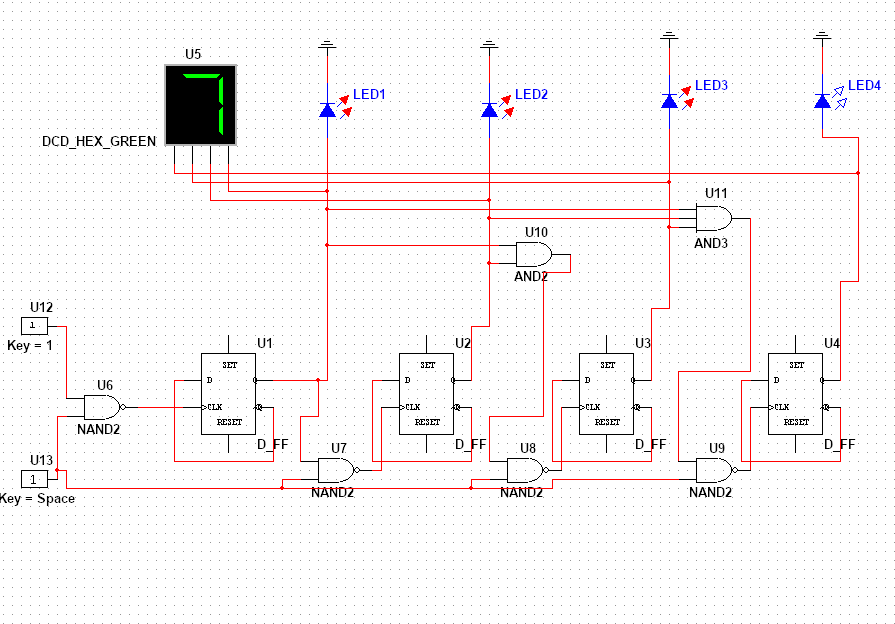
\includegraphics[width=\linewidth]{img/sc6.png}
    \caption{Схема шестнадцатеричного счетчика.}
    \label{sc6}
\end{figure}

\begin{figure}[ht]
    \centering
    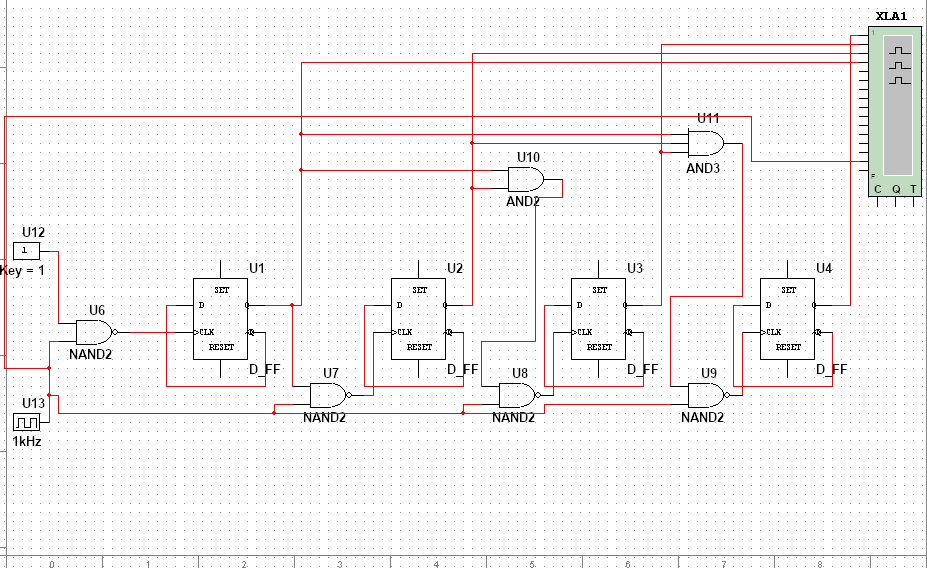
\includegraphics[width=\linewidth]{img/sc7.png}
    \caption{Схема шестнадцатеричного счетчика с логическим анализатором.}
    \label{sc7}
\end{figure}

\begin{figure}[ht]
    \centering
    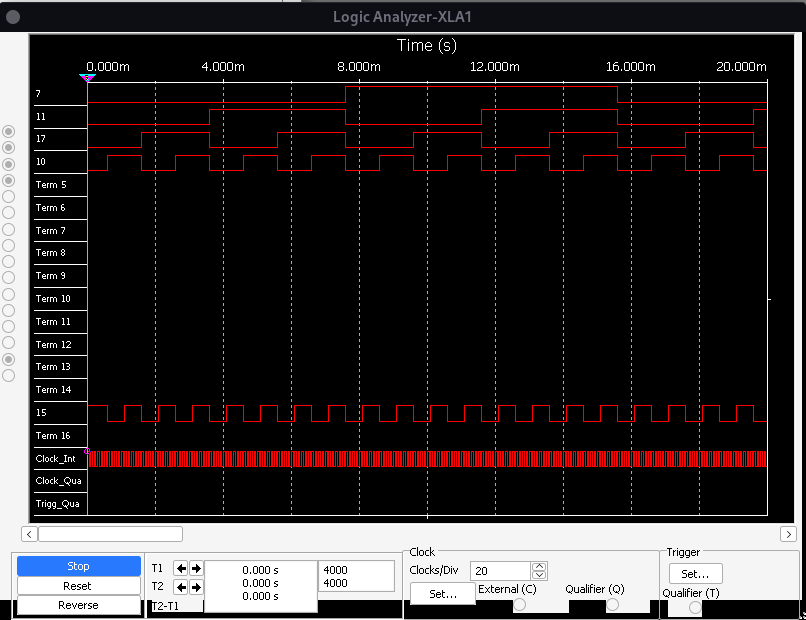
\includegraphics[width=\linewidth]{img/sc8.png}
    \caption{Временные диаграммы шестнадцатеричного счетчика.}
    \label{sc8}
\end{figure}


\clearpage

\section{Исследование четырёхразрядного синхронного суммирующего счётчика с параллельным переносом ИС К555ИЕ9}

Схема на рисунке \ref{sc9} дает управление одиночными импульсами.

\begin{figure}[ht]
    \centering
    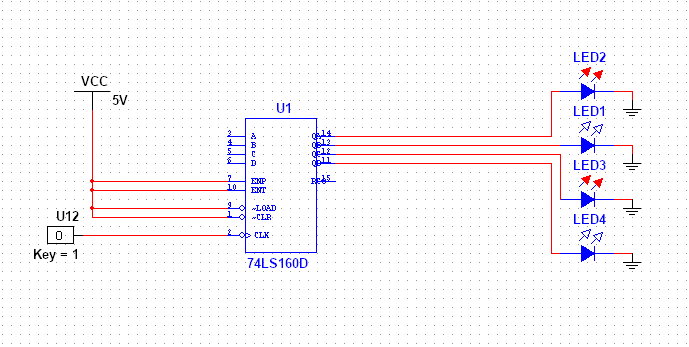
\includegraphics[width=\linewidth]{img/sc9.png}
    \caption{Четырехразрядный суммирующий счетчик с одним меняющимся входом.}
    \label{sc9}
\end{figure}

\begin{figure}[ht]
    \centering
    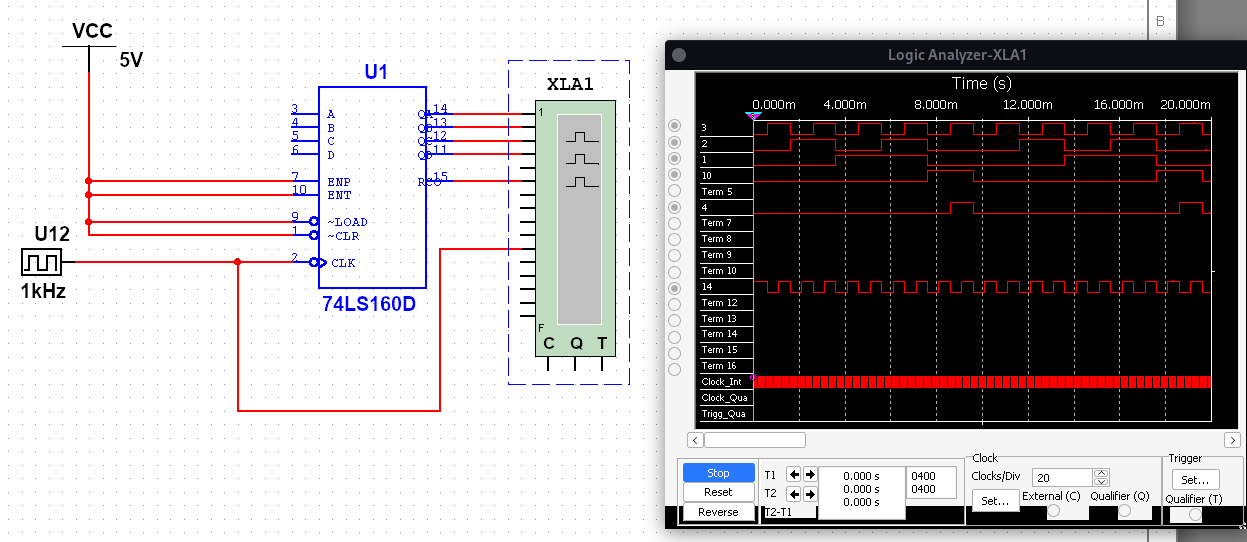
\includegraphics[width=\linewidth]{img/sc10.png}
    \caption{Четырехразрядный суммирующий счетчик с управлением импульсами генератора.}
    \label{sc10}
\end{figure}

\clearpage

\section{Исследование схем наращивания разрядности счётчиков ИЕ9 до четырех секций с последовательным переносом между секциями и по структуре «быстрого» счёта}

Ниже, на рисунке \ref{sc11}, представлен многоразрядный десятичный счетчик.

\begin{figure}[ht]
    \centering
    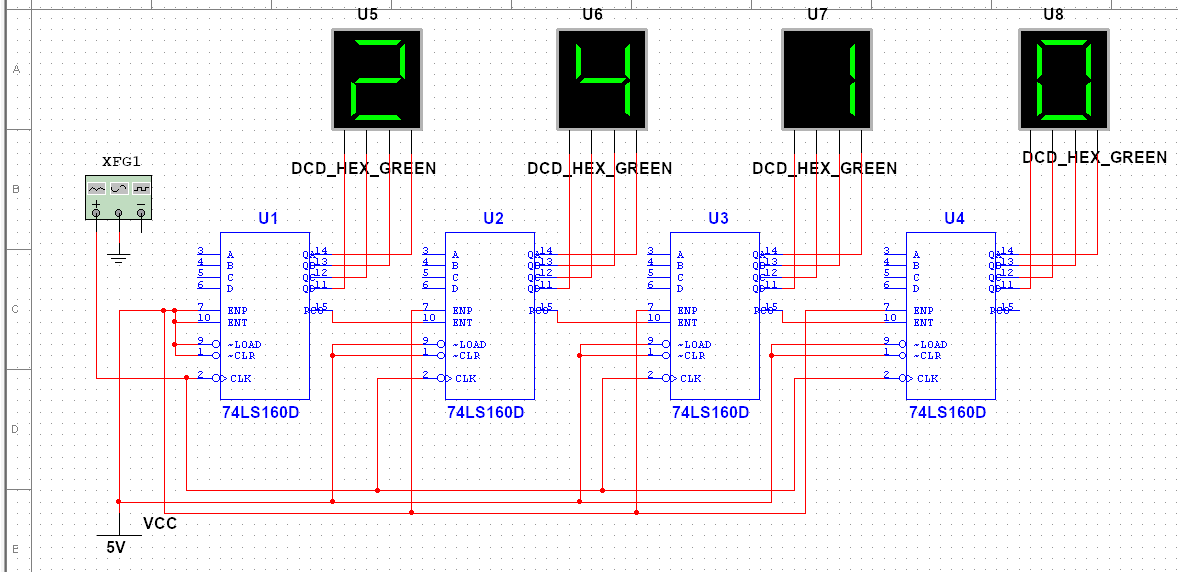
\includegraphics[width=\linewidth]{img/sc11.png}
    \caption{Четырехразрядный суммирующий счетчик с управлением импульсами генератора.}
    \label{sc11}
\end{figure}
